\chapter{(OLD) Beyond SBDRL (to be converted over)}
%%%%%%%%%%%%%%%%%%%%%%%%%%%%%%%%%%%%%%%%%%%%%%%%%%%%%%%%%%%%%%%%%%%%%%%%%%%%%
\section{Worlds without inverse actions}

%%%%%%%%%%%%%%%%%%%%%%%%%%%%%%%%%%%%%%%%%%%%%%%%%%%%%%%%%%%%%%
\subsection{Example 3: irreversible inhomogeneous actions}

\begin{remark}
    Considering this example, we note that the irreversible action moves from one `reversible plane' to another.
    Perhaps we can treat an irreversible action as having a `reversible action affecting part' and a `world affecting part'; in this example, the reversible action affecting part would be the identity action since the reversible action network is unchanged by the irreversible action.
\end{remark}

%%%%%%%%%%%%%%%%%%%%%%%%%%%%%%%%%%%%%%%%%%%%%%%%%%%%%%%%%%%%%%%%%%%%%%%%%%%%%%
\section{Worlds without inverse actions or unrestricted actions}\label{sec:Worlds without inverse actions or unrestricted actions}

\begin{proposition}\label{prp:all_worlds_give_small_category_action}
    Consider a world $\mathscr{W}$ with a set $W$ of world states and containing an agent with a set $A$ of actions.
    $*: (A/\sim) \times W \to W'$, where $W' \subseteq W$, is the action of a small category $A/\sim$ on $W$.
\end{proposition}
\begin{proof}
    (1) Associativity of $A/\sim$ is given by proposition ref[prp:Asim-associative].
    (2) Identity element of $A/\sim$ is given by proposition ref[prp:Asim-identity].
    Since $A/\sim$ satisfies properties (1) and (2), $A/\sim$ is a small category.
    Therefore $*$ is the action of a small category.
\end{proof}

\begin{remark}
    We can consider two equivalent perspectives of $*$:
    \begin{enumerate}
        \item $A/\sim$ is a small category and $*$ is a full action of $A/\sim$ on $W$.
        \item $A/\sim$ is a monoid and $*$ is a partial action of $A/\sim$ on $W$.
    \end{enumerate}
\end{remark}

%%%%%%%%%%%%%%%%%%%%%%%%%%%%%%%%%%%%%%
\subsection{Example 2: irreversible action-inhomogeneous world}\label{sec:masked irreversible action-inhomogeneous world}

We will now apply the masking treatment of restricted actions to the world $\mathscr{W}_{consumable}$ (see Figure \ref{fig:consumable_world_states} for world states); for example, if $\mathscr{W}_{consumable}$ is not in state $w_{1}$ then the consume action is undefined.

\begin{figure}[H]
    \centering
    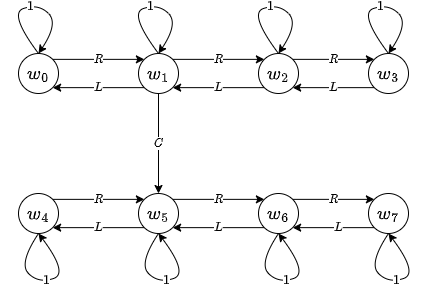
\includegraphics[scale=0.5]{5BeyondSBDRL/Old/Images/fig-min-action-net-world-with-consumable-masked.png}
    \caption{Minimum action network for world containing an agent and a consumable.}
    \label{fig-min-action-net-world-with-consumable-masked}
\end{figure}

The action Cayley table for $\mathscr{W}_{consumable}$ with the masked treatment of the walls contains 20 elements.
As shown in Table \ref{tab:masked-consumable-properties}, $A/\sim$ is a small category.

\begin{table}[H]
    \centering
    \begin{tabular}{c|c}
        \textbf{Property}   & \textbf{Present?} \\
        \hline
        Totality            & N\\
        Identity            & Y\\
        Inverse             & N\\
        Associative         & Y\\
        Commutative         & N
    \end{tabular}
    \caption{Properties of the $A/\sim$ algebra.}
    \label{tab:masked-consumable-properties}
\end{table}








-------------

\begin{remark}
    \draftnote{blue}{Consider}{
    Make this about state Cayley tables ?
    }
    For any world, once the agent has the state Cayley table for any initial world state it can produce the state Cayley table for any other initial world state by applying an action that transitions from the old initial world state to the new initial world state to every element of the action Cayley table.
\end{remark}

\draftnote{blue}{To do}{
Can we prove something about this?
e.g., 
}
We have also demonstrated that neither the identity treatment nor the masked treatment produces the more simple algebra in every world.
For $\mathscr{W}_{wall}$, the identity treatment contains fewer elements than the masked treatment (26 elements vs 59 elements), while for $\mathscr{W}_{consumable}$ the masked treatment contains fewer elements than the identity treatment (20 elements vs 64 elements).



%%%%%%%%%%%%%%%%%%%%%%%%%%%%%%%%%%%%%%%%%%%%%%%
\chapter{Action-homogeneous worlds and generalisation potential}

\draftnote{blue}{awjdean}{
Hypothesis: action-homogeneous worlds are easier to learn.
Can we design a method that an agent could use to work out the algebra for these worlds ?
Could use the (old) algorithm we developed because each time we move to a new state it's as if we're returning to where we began (kinda - states are still distinct).
}


\whendraft{
	\begin{proposition}
		If $A/\sim$ is a group, then $a' \circ a * w = w$ ($w \in W$, $a, a' \in A/\sim$) does not mean that $a' \circ a * w' = w'$ for all $w' \in W$.
	\end{proposition}
	\begin{proof}
		Proof by counter example.
		Consider the world given in Figure ?
		[insert figure here]
		The algebra of the actions of an agent with minimum actions $\{1, a, b\}$ is given by the following action Cayley table:
		[insert action Cayley table]
	\end{proof}
}

\begin{world_condition}[Action homogeneity]\label{wldcon:action-homogeneity}
	For every pair $(w_{1}, w_{2}) \in W^{2}$, there exists a bijective map $\sigma_{(w_{1},w_{2})}: W \to W$ such that $\sigma_{(w_{1},w_{2})}(w_{1})=w_{2}$ and such that:

	\begin{enumerate}
		\item for every $d \in D_{A}$ with $d: s(d) \xrightarrow{a} t(d)$, there exists a $d' \in D_{A}$ with $d': \sigma_{(w_{1}, w_{2})}(s(d)) \xrightarrow{a} \sigma_{(w_{1}, w_{2})}(t(d))$;

		      % Is this part needed --> implied by first condition due to $\sigma$ being a bijection ?
		\item for every $d \in D_{A}$ with $d: s(d) \xrightarrow{a} t(d)$, there exists a $d' \in D_{A}$ with $d': \sigma^{-1}_{(w_{1}, w_{2})}(s(d)) \xrightarrow{a} \sigma^{-1}_{(w_{1}, w_{2})}(t(d))$.
	\end{enumerate}
\end{world_condition}

World condition ref[wldcon:action-homogeneity] means that action sequences have the same result for any initial world state.
Essentially, this means that the world looks the same from any world state with respect to the relationships of actions.
We call worlds with world condition ref[wldcon:action-homogeneity] \textit{action-homogeneous worlds}.

\begin{definition}[Weak equivalence $\sim_{w}$]\label{def:weak action equivalence}
	For $a,a' \in A$ and $w \in W$, $a \sim_{w} a$ if $a * w = a' * w$ or $a$ and $a'$ are both restricted actions with respect to $w$.
\end{definition}

\begin{remark}
	In definition \ref{def:weak action equivalence}, for the case where $a, a'$ are both restricted actions, then we say $a * w = a' * w$.
	The meaning of $a * w$ where $a$ is restricted on $w$ will be defined later.
\end{remark}

\begin{proposition}
	$\sim_{w}$ is an equivalence relation.
\end{proposition}
\begin{proof}
	To show that $\sim_{w}$ is an equivalence relation, we need to show that the relation is (a) reflexive, (b) transitive, and (c) symmetric.
	(a) For a binary relation $R$ over a set $X$ to be reflexive: $x R x$ for every $x \in X$.
	For $w \in W$, if $a * w$ is defined then $a * w = a * w$ from the properties of $=$ for any $a \in A$.
	Therefore, $a \sim_{w} a$.
	(b) For a binary relation $R$ over a set $X$ to be transitive: if $a R b$ and $b R c$ then $a R c$ for all $a,b,c \in X$.
	If $a \sim_{w} a'$ and $a' \sim_{w} a''$, then $a * w = a' * w$, $a' * w = a'' * w$ for all $w \in W$.
	Combining these two equations gives $a * w = a'' * w$.
	(c) For a binary relation $R$ over a set $X$ to be reflexive: if $a R b$, then $b R a$ for all $a,b \in X$.
	If $a \sim_{w} a'$, then $a * w = a' * w$. Therefore $a' * w = a * w$, and so $a' \sim_{W} a$.
\end{proof}

For action-homogeneous worlds, the following properties hold:
\begin{enumerate}
	\item If a world is action-homogeneous, then $a \sim_{w} a'$ means $a \sim a'$ - this makes it much easier to learn the algebra of action-homogeneous worlds;

	\item The number of elements in $A/\sim$ is always equal to the number of states in the world since for any state $w \in W$, there is exactly one action $a \in A/\sim$ for which $a * w = w'$ where $w'$ is any state in $W$; therefore the number of elements in the action algebra is equal to the number of states in $W$;

	\item If $a * w_{i} = w_{j}$, then there exists a world state $w_{k} \in W$ such that $a * w_{k} = w_{i}$.
	      In other words, if $a$ is defined from one world state it is defined from all world states;

	\item If $a' * (a * w) = a * (a' * w) = w$ for any $w \in W$, then $a' * (a * w) = a * (a' * w) = w$ for all $w \in W$.
	      In other words, reversible actions imply inverse actions.
\end{enumerate}

\whendraft{
	\textbf{[Insert info about generalisation.]}
	\begin{itemize}
		\item If we know that, from a particular initial state, a particular sequence of actions has a particular outcome and we know that a different sequence of actions from the same initial state has the same outcome then we know that those two action sequences will have the same outcome in from every initial state (and therefore will be equivalent?!).
		      \begin{itemize}
			      \item Illustrate this using the counter-example - see PhD Notebook 1 notes.
		      \end{itemize}
	\end{itemize}
}

